\documentclass{article}
\usepackage[preprint]{style/neurips_2020}
\usepackage{hyperref}
\usepackage{tikz}
\newif\ifcomment\commenttrue
% Preamble file contains handy macros and most packages you might want to use.
% At the start are packages that conflict with various styles.  Don't add them
% in!  Just put it in your main TeX file instead.

% Do not put either of these (subfigure or subfloat) into the preamble
% - they clash.  Use them in the final LaTeX document
% \usepackage{subfigure}
% \suepackage{subfloat}

% Do not use times in the preamble!  It just causes problems with some
% publication chairs (e.g., ICML 2013).  If you want it, put it in your own
% document.
% \usepackage{times}


% Breaks ACM-SIG style
% \usepackage{titlesec}
% \usepackage{amsthm}
% \usepackage{nomencl}

% comment out the following line, as it conflicts with aistats2012.sty
%\usepackage{caption}

% This is required by NSF.  Do not remove; if it conflicts with
% another package, fix that problem without removing this from
% Preamble.
% Unless for AAAI ... this needs a new bibfile that plays well with hyperref.
%\usepackage[a-1b]{pdfx}

% Below should be safe
\usepackage{framed}
\usepackage{mdwlist}
\usepackage{latexsym}
\usepackage{colortbl}
\usepackage{xcolor}
\usepackage{nicefrac}
\usepackage{booktabs}
\usepackage{amsfonts}
\usepackage[T1]{fontenc}
\usepackage{bold-extra}
\usepackage{amsmath}
\usepackage{amssymb}
\usepackage{bm}
\usepackage{graphicx}
\usepackage{mathtools}
\usepackage{microtype}
\usepackage{multirow}
\usepackage{multicol}
% Don't use hyperref or url, as it can screw up AAAI / ICML formatting
%\usepackage{url}
\usepackage{latexsym,comment}
\usepackage[normalem]{ulem}

\newcommand{\breakalign}{\right. \nonumber \\ & \left. \hspace{2cm}}



\newcommand{\feat}[1]{{\small \texttt{#1}}}
\newcommand{\act}[1]{{\small \texttt{#1}}}
\newcommand{\ngram}[0]{$n$-gram}
\newcommand{\topic}[1]{\underline{#1}}
\newcommand{\gem}[1]{\mbox{\textsc{gem}}}
\newcommand{\abr}[1]{\textsc{#1}}
\newcommand{\camelabr}[2]{{\small #1}{\textsc{#2}}}
\newcommand{\abrcamel}[2]{{\textsc #1}{\small{#2}}}
\newcommand{\grammar}[1]{{\color{red} #1}}
\newcommand{\explain}[2]{\underbrace{#2}_{\mbox{\footnotesize{#1}}}}
\newcommand{\dir}[1]{\mbox{Dir}(#1)}
\newcommand{\bet}[1]{\mbox{Beta}(#1)}
\newcommand{\py}[1]{\mbox{\textsc{py}}(#1)}
\newcommand{\td}[2]{\mbox{\textsc{TreeDist}}_{#1} \left( #2 \right)}
\newcommand{\yield}[1]{\mbox{\textsc{Yield}} \left( #1 \right)}
\newcommand{\mult}[1]{\mbox{Mult}( #1)}
\newcommand{\wn}{\textsc{WordNet}}
\newcommand{\twentynews}{\textsc{20news}}
\newcommand{\g}{\, | \,}
\newcommand{\Gam}[1]{\Gamma \left( \textstyle #1 \right)}
\newcommand{\LG}[1]{\log \Gamma \left( \textstyle #1 \right)}
\newcommand{\Pois}[1]{\mbox{Poisson}(#1)}
\newcommand{\pcfg}[3]{#1_{#2 \rightarrow #3}}
\newcommand{\grule}[2]{#1 \rightarrow #2}
\newcommand{\kl}[2]{D_{\mbox{\textsc{KL}}} \left( #1 \,||\, #2 \right)}

\newcommand{\digambig}[1]{\Psi \left( #1 \right) }
\newcommand{\digam}[1]{\Psi \left( \textstyle #1 \right) }
\newcommand{\ddigam}[1]{\Psi' \left( \textstyle #1 \right) }


\renewenvironment{quote}
               {\list{}{\rightmargin\leftmargin}%
                \item\relax\small\ignorespaces}
               {\unskip\unskip\endlist}

\DeclareMathOperator*{\argmax}{arg\,max}
\DeclareMathOperator*{\argmin}{arg\,min}
\newcommand{\bmat}[1]{\text{\textbf{#1}}}
\newcommand{\bvec}[1]{\boldsymbol{#1}}

%\newcommand{\email}[1]{ {\small \href{mailto://#1}{\texttt{#1} }  }}
\newcommand{\emaillink}[1]{ {\small \href{mailto://#1}{\texttt{#1}}}}
\newcommand{\smallemaillink}[2]{ {\small \href{mailto://#2}{\texttt{#1}}}}

% JBG: Consider renaming from \ch to \zh because of conflict when adding Cyrillic
\newcommand{\ch}[1]{\begin{CJK*}{UTF8}{gbsn}#1\end{CJK*}}

\newcommand{\e}[2]{\mathbb{E}_{#1}\left[ #2 \right] }
\newcommand{\h}[2]{\mathbb{H}_{#1}\left[ #2 \right] }
\newcommand{\ind}[1]{\mathds{1}\left[ #1 \right] }
\newcommand{\ex}[1]{\mbox{exp}\left\{ #1\right\} }
\newcommand{\D}[2]{\frac{\partial #1}{\partial #2}}
\newcommand{\elbo}{\mathcal{L}}

\newcommand{\hidetext}[1]{}
\newcommand{\ignore}[1]{}

\newcommand{\todo}[1]{\textcolor{red}{{\bf TODO: #1}}}

\ifcomment
\newcommand{\pinaforecomment}[3]{\colorbox{#1}{\parbox{.8\linewidth}{#2: #3}}}
\else
\newcommand{\pinaforecomment}[3]{}
\fi

\newcommand{\jbgcomment}[1]{\pinaforecomment{red}{JBG}{#1}}
\newcommand{\mjpcomment}[1]{\pinaforecomment{blue}{MJP}{#1}}
\newcommand{\czcomment}[1]{\pinaforecomment{orange}{chen}{#1}}
\newcommand{\ffcomment}[1]{\pinaforecomment{red}{FF}{#1}}
\newcommand{\fpcomment}[1]{\pinaforecomment{green}{FP}{#1}}
\newcommand{\yhcomment}[1]{\pinaforecomment{green}{YH}{#1}}
\newcommand{\hhecomment}[1]{\pinaforecomment{blue}{HH}{#1}}
\newcommand{\tncomment}[1]{\pinaforecomment{blue}{TN}{#1}}
\newcommand{\mnicomment}[1]{\pinaforecomment{green}{Mohit}{#1}}
\newcommand{\prcomment}[1]{\pinaforecomment{lightblue}{Pedro}{#1}}
\newcommand{\fscomment}[1]{\pinaforecomment{orange}{Shi}{#1}}
\newcommand{\vmcomment}[1]{\pinaforecomment{yellow}{Varun}{#1}}
\newcommand{\rscomment}[1]{\pinaforecomment{yellow}{Richard}{#1}}
\newcommand{\jszcomment}[1]{\pinaforecomment{green}{JSG}{#1}}
\newcommand{\ascomment}[1]{\pinaforecomment{blue}{AS}{#1}}
\newcommand{\vecomment}[1]{\pinaforecomment{blue}{VE}{#1}}
\newcommand{\halcomment}[1]{\pinaforecomment{magenta!20}{Hal}{#1}}
\newcommand{\kgcomment}[1]{\pinaforecomment{blue}{Kim}{#1}}
\newcommand{\vancomment}[1]{\pinaforecomment{green}{VAN}{#1}}
\newcommand{\thangcomment}[1]{\pinaforecomment{green}{Thang}{#1}}
\newcommand{\alvincomment}[1]{\pinaforecomment{cyan}{Alvin}{#1}}
\newcommand{\reviewercomment}[1]{\pinaforecomment{blue}{Reviewer}{#1}}
\newcommand{\brscomment}[1]{\pinaforecomment{blue}{BRS}{#1}}
\newcommand{\psrcomment}[1]{\pinaforecomment{yellow}{PSR}{#1}}
\newcommand{\zkcomment}[1]{\pinaforecomment{cyan}{ZK}{#1}}
\newcommand{\swcomment}[1]{\pinaforecomment{yellow}{SW}{#1}}
\newcommand{\shaycomment}[1]{\pinaforecomment{yellow}{SBC}{#1}}
\newcommand{\jlundcomment}[1]{\pinaforecomment{cyan}{J}{#1}}
\newcommand{\kdscomment}[1]{\pinaforecomment{ceil}{KDS}{#1}}
\newcommand{\lkfcomment}[1]{\pinaforecomment{yellow}{LF}{#1}}
\newcommand{\yfcomment}[1]{\pinaforecomment{brown}{YF}{#1}}
\newcommand{\ewcomment}[1]{\pinaforecomment{lightblue}{Eric}{#1}}
\newcommand{\pgcomment}[1]{\pinaforecomment{cyan}{Pranav}{#1}}
\newcommand{\bencomment}[1]{\pinaforecomment{lightblue}{Ben}{#1}}

\newcommand{\smalltt}[1]{ {\tt \small #1 }}
\newcommand{\smallurl}[1]{ \begin{tiny}\url{#1}\end{tiny}}
%\newcommand{\smallurl}[1]{ \begin{tiny} HIDDEN \end{tiny}}
\newenvironment{compactenum}{ \begin{enumerate*} \small }{ \end{enumerate*} }

\definecolor{lightblue}{HTML}{3cc7ea}
\definecolor{CUgold}{HTML}{CFB87C}
\definecolor{grey}{rgb}{0.95,0.95,0.95}
\definecolor{ceil}{rgb}{0.57, 0.63, 0.81}
\definecolor{UMDred}{HTML}{ed1c24}
\definecolor{UMDyellow}{HTML}{ffc20e}

% Datasets / Models

\newcommand{\qb}[0]{Quizbowl}
\newcommand{\qa}[0]{\abr{qa}}
\newcommand{\triviaqa}{\camelabr{Trivia}{qa}}
\newcommand{\searchqa}{\camelabr{Search}{qa}}
\newcommand{\qblink}{\abrcamel{qb}{Link}}
\newcommand{\qanta}{\textsc{qanta}}
\newcommand{\muse}{\textsc{muse}}
\newcommand{\squad}{\textsc{sq}{\small u}\textsc{ad}}
\newcommand{\fever}{\abr{fever}}
\newcommand{\quac}{\textsc{q}{\small u}\textsc{ac}}
\newcommand{\elmo}{\textsc{elm}{\small o}}
\newcommand{\fone}{$F_1$}
\newcommand{\jeopardy}{\textit{Jeopardy!}}
\newcommand{\dan}[0]{\abr{dan}}
\newcommand{\lstm}[0]{\abr{lstm}}
\newcommand{\gru}[0]{\abr{gru}}
\newcommand{\ibm}[0]{\abr{ibm}}
\newcommand{\nquestions}[0]{119,093}
\newcommand{\ntotalquestions}[0]{132,849}
\newcommand{\nsentences}[0]{440,195}
\newcommand{\wikidumpdate}[0]{4/18/2018}
\newcommand{\simplequestions}[0]{SimpleQuestions}
\newcommand{\protobowl}[0]{Protobowl}

\newcommand{\coqa}{\textsc{c}{\small o}\textsc{qa}}
\newcommand{\cove}{\textsc{c}{\small o}\textsc{v}{\small e}}
\newcommand{\nel}[0]{\abr{nel}}
\newcommand{\quel}[0]{\abr{quel}}
\newcommand{\rover}[0]{\abr{rover}}
\newcommand{\opendialkg}{\abr{o}{\small pen}\abr{d}{\small ial}\abr{kg}}
\newcommand{\mrr}{\abr{mrr}}
\newcommand{\tfidf}{\abr{tf-idf}}
\newcommand{\hre}{\abr{hre}}
\newcommand{\parlai}{\abr{p}{\small arl}\abr{ai}}
\newcommand{\wow}{\abr{w}{\small o}\abr{w}}
\newcommand{\bilstm}{\abr{b}{\small i}\abr{lstm}}
\newcommand{\tqa}{\abr{t}{\small rivia}\abr{qa}}
\newcommand{\cis}{\textsc{cis}}
\newcommand{\ir}{\abr{ir}}
\newcommand{\rc}{\abr{rc}}
\newcommand{\rnn}{\abr{rnn}}
\newcommand{\trec}{\abr{trec}}
\newcommand{\babi}{{\small b}\abr{a}{\small b}\abr{i}}

\graphicspath{{2020_tacl_qbnel/commit_fig/}{2020_tacl_qbnel/autofig/}{2020_tacl_qbnel/figures/}}

\title{What more can Entity Linking do for Question Answering?}

\author{Naveen Raman \\
	University of Maryland \\
	\texttt{nraman1@umd.edu} \\
	\And
	Pedro Rodriguez \\
	University of Maryland \\
	\texttt{pedro@cs.umd.edu} \\
	\And
	Jordan Boyd-Graber \\
	University of Maryland \\
	\texttt{jbg@umiacs.umd.edu} \\
}

\begin{document}

\maketitle

\begin{abstract} 
	\begin{abstract}

In additon to the traditional task of getting machines to answer
questions, a major research question in question answering is to create interesting,
challenging questions that can help systems learn how to answer
questions and also reveal which systems are the best at answering
questions.
We argue that creating a question answering dataset---and
the ubiquitous leaderboard that goes with it---closely resembles
running a trivia tournament: you write questions, have agents (either
humans or machines) answer the questions, and declare a winner.
However, the research community has ignored the decades of hard-learned
lessons from decades of the trivia community creating vibrant, fair,
and effective question answering competitions.
After detailing problems with existing QA datasets, we outline the key lessons---removing ambiguity, discriminating skill,
and adjudicating disputes---that can transfer to QA research and
how they might be implemented for the QA community.


\end{abstract}

\end{abstract}
% intro

\section{Orthogonal Cross-Lingual Mappings}\label{sec:intro}

Cross-lingual word embedding (\abr{clwe}) models map words from
multiple languages to a shared vector space, where words with similar
meanings are close, regardless of language.
\abr{clwe} is widely used in multilingual natural language
processing~\citep{klementiev-12,guo-15,zhang-16}.
Recent \abr{clwe} methods~\citep{ruder-17,glavas-19} independently train two
monolingual embeddings on large monolingual corpora and then align them
with a linear transformation.
Previous work argues that these transformations should be
\emph{orthogonal}~\citep{xing-15,smith-17,artetxe-16}: for any two words, the
dot product of their representations is the same as the dot product with the
transformation.
This preserves similarities and substructure of the original monolingual word
embedding but enriches the embeddings with multilingual connections between
languages.

\begin{figure*}[!t]
  \centering
  \includegraphics[width=.8\linewidth]{\figfile{girl.pdf}}
  \caption{The most similar Japanese words for \ja{少女} (sh\={o}jo ``girl'')
  and English words for ``girl'', measured by cosine similarity on Wikipedia
  fastText vectors, before (left) and after (right) \name{}.
  In the original embedding spaces, ``boy'' is the nearest neighbor for both
  languages but with a very different cosine similarity, and ``cat'' in English
  is not close to ``girl'': both violate the isomorphism assumed by an
  orthogonal transformation for cross-lingual representations.
  \name{} replaces \ja{猫} (neko ``cat'') with the more
  relevant \ja{美少女} (bish\={o}jo ``pretty girl'') and brings cosine similarities 
  closer.}
  \label{fig:example}
\end{figure*}

Thus, many state-of-the-art mapping-based \abr{clwe} methods impose an
orthogonal
constraint~\citep{artetxe-17,conneau-18,alvarez-18,artetxe-18b,ruder-18,alvarez-19}.
The success of orthogonal methods relies on the assumption that embedding spaces
are isomorphic; i.e., they have the same inner-product structures across
languages, but this does not hold for all
languages~\citep{sogaard-18,fujinuma-19}.
For example, English and Japanese fastText vectors~\citep{bojanowski-17} have
different substructures around ``girl'' (Figure~\ref{fig:example} left).
As a result, orthogonal mapping fails on some languages---when
\citet{hoshen-18} align fastText embeddings with orthogonal mappings, they
report 81\% English--Spanish word translation accuracy but only 2\% for the
more distant English--Japanese.

While recent work challenges the orthogonal
assumption~\citep{doval-18,joulin-18,jawanpuria-19}, we focus on whether simple
preprocessing techniques can \emph{improve the suitability of orthogonal
models}.
Our iterative method normalizes monolingual embeddings to make their structures
more similar (Figure~\ref{fig:example}), which improves subsequent
alignment.

Our method is motivated by two desired properties of monolingual embeddings
that support orthogonal alignment:
\begin{enumerate*}
\item Every word vector has the same length.
\item Each language's mean has the same length.
\end{enumerate*}
Standard preprocessing such as dimension-wise mean centering and length
normalization~\cite{artetxe-16} do not meet the two requirements at
the same time.
%
Our analysis leads to \emph{\name{}}, an alternating projection
algorithm that normalizes any word embedding to provably satisfy both
conditions.
%
After normalizing the monolingual embeddings, we then apply
mapping-based \abr{clwe} algorithms on the transformed embeddings.

We empirically validate our theory by combining \name{} with three
mapping-based \abr{clwe} methods.
%
\name{} improves word translation accuracy on a dictionary induction benchmark
across thirty-nine language pairs.

\section{Noun Phrase Linking}
\label{sec:gen}
We define the problem of Noun Phrase Linking and motivate the problem by discussing the improved performance in downstream tasks due to noun phrase linking. 
We additionally define guidelines for noun phrase linking and develop an interface for annotating documents using those guidelines in Section 3. 

\subsection{Noun Phrase Linking}
Named entities refer to specific nouns such as people's names, and the name of places. 
Annotating named entities provides a gain in accuracy when augmented to QA systems, but named entities exclude certain noun phrases that could further assist QA systems. 
In particular, resolving anaphoric references, such as resolving "One work by this author" to "Novum Organum", provides a more difficult task because of the lack of a direct link between the noun phrase and the entity to be linked. 
Resolving anaphoric references could allow for a bigger gain in helping QA systems, as seen by changing the answer to the correct answer, Francis Bacon, when noun phrases are replaced by their referenced entity (Figure 1).  
\\
\\
We define the task of noun phrase linking to be the union of annotating anaphoric references along with annotating named entities, and in effect, annotating all noun phrases in a document that link to a named entity.
This task differs from the coreference and entity linking, as entities that are referred to, but not necessarily ever mentioned in the document, can be linked. 
For example, within the first sentence of Figure 1, Novum Organum is never mentioned. 
However, "One work by this author" refers to Novum Organum, and so would be annotated in Noun Phrase Linking, but not in either coreference or entity linking.  
We develop guidelines for linking noun phrases (Section \ref{sec:int}), and plan to conduct experiments to determine the effect of annotating noun phrases upon QA performance (Section \ref{sec:exp}). 
\\
\\
We extend traditional entity linking to noun phrase linking because traditional entity linkers have been shown to perform well on \nel{} tasks, and extending to noun phrase linking allows for a more challenging task. 
Current models do well in NEL and coreference resolution, both of which are tasks related to noun phrase linking. 
Thus, it's plausible, although imperfect, that future models may show improvement on downstream tasks. 
We also propose experiments that explore the effect that noun phrase linking has upon question answering accuracy (Section \ref{sec:exp}), to determine the extent to which noun phrase linking assists question answering systems. 
 

\subsection{Noun Phrase Linking Guidelines}
We develop guidelines for determining which entities to link, and what to link them to. 
These guidelines will be used by annotators, along with examples, when determining what to annotate. 
We link text spans that are noun phrases and refer to a uniquely identifiable named entity in the knowledge base. 
For example, in Figure 1, we link "idols of the theatre" because it refers to a named entity. 
On the other hand, we don't link the word "symbols", despite the presence of a Wikipedia page for symbol, because smybol does not refer to a specific symbol, but rather the general word. 
If no Wikipedia page is present for a noun phrase, then we link it with "No Entity."
The "No Entity" links are subdivided into "No Entity Character" and "No Entity Literature" for characters and works of literature respectively.
Wikipedia is an incomplete knowledge base; rather than omit links simply because the correct entity does not exist, the entity should be linked, but assigned to a special null entity indicating its type. 




\section{Data Collection}
\label{sec:int}

The task of noun phrase linking is more difficult than \nel{}, due to the difficulty of finding indirect links.  Because of this, we develop methods to efficiently collect data.
The Quizzical Entity Linking (\quel{}) dataset is annotated with an interface (Figure~\ref{fig:nel-int}) that supports basic entity linking functionality (Section~\ref{sec:el-int}), configurable inclusion of machine-generated links to vary annotation conditions, and features to motivate expert annotators to participate in data collection (Section~\ref{sec:packet}).
Gold data will be collected by the authors of this paper (Section~\ref{sec:gold}), and all other data will be collected by organizers of \qb{} tournaments (Section~\ref{sec:expert}).
We plan to utilize human-in-the-loop annotation to help annotators and speed up the annotation process (Section~\ref{sec:active}) and assist users by pre-linking certain entities (Section~\ref{sec:other-ent}). 

\subsection{Entity Linking Interface}
\label{sec:el-int}

To collect the \quel{} dataset we built the interface in Figure~\ref{fig:nel-int}.
To annotate entity links, users: (1) select a text span, (2) search for the correct entity, and (3) confirm their choice.
Annotators select entities from among all valid Wikipedia pages.\footnote{
    We use the Wikipedia dump from 06/2020.
}
This process is iterative until the user is satisfied with the links in the question.
Currently, we suggest entities for the user based on full-text search, matching their noun phrase to Wikipedia articles. 


\begin{figure}[t]
    \centering
    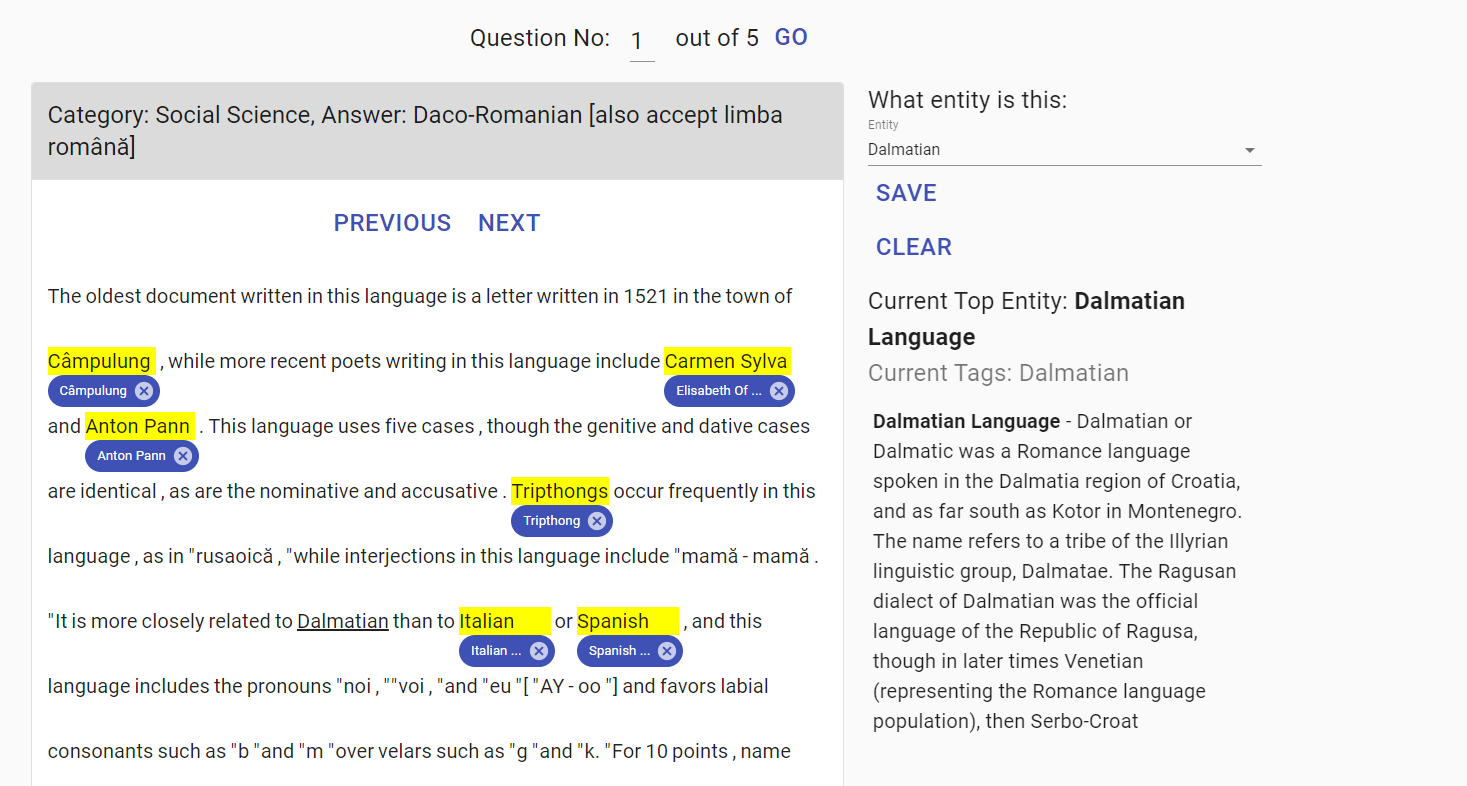
\includegraphics[width=\columnwidth]{quel-interface}
    \caption{
        We show our annotation interface currently, which has the ability to select text spans and tag them with an entity. 
        We plan to suggest noun phrases to annotate in the future, and also plan to allow users to annotate nested spans. 
    }
    \label{fig:nel-int}
\end{figure}


We plan to add annotations for subspans, otherwise known as nested entities. 
Examples of this include the entity "Washington crossing the Delaware"; the whole entity would be matched with the painting, while Washington would be linked to George Washington and Delaware would be linked to Delaware. 
We propose two methods of doing this
\begin{enumerate}
	\item List of noun phrase suggestions, which includes nested noun phrases. 
	The user simply has to annotate each noun phrase. This would reduce the time needed for annotation, as the user does not need to search for noun phrases. 
	\item Augment the current interface with nested spans, allowing users to tag a particular word or phrase as part of multiple entities. 
	While simpler to implement, this option might be less user friendly. 
\end{enumerate}




\subsection{Using other Entity Linkers}
\label{sec:other-ent} 
We utilize different experimental conditions to speed up the entity linking process by pre-populating entity links. 
Later (Section~\ref{sec:exp}), we propose experiments to compare different experimental conditions to determine which condition would optimize entity linking accuracy and speed. 
Before a question is loaded, we assign the annotator an experimental condition that decides how entity links are pre-populated.
In the first condition, no entity links are pre-populated so the question is annotated from scratch.
The second condition pre-populates entity links with the output of one randomly selected entity linker. 
In the third condition, we use a named entity recognition system to display candidate mentions, but do not pre-link them to Wikipedia entities.
The final condition pre-populates links that are predicted by two or more of the linkers.
Later, we analyze the annotation differences on a shared set of questions as well as distributionally across the non-shared questions.

\subsection{Human-in-the-Loop Annotation}
\label{sec:active} 
Prior research has shown that human-in-the-loop annotation for entity linking tasks can speed up the process~\cite{klie2020hero}. 
To do this, we plan to recommend which entities a particular noun phrase might be linked to via a model, so that  our annotation system assists users with determining what noun phrased are linked to. 
At the moment, we plan to build two simple baseline models. 
The first model recognizes noun phrases based off of n-grams, though we could also use some type of BERT based embedding~\cite{devlin2018bert}. 
The second model uses these noun phrases and links them to a Wikipedia page. 
The model will deliver a confidence score for a list of entities associated with each noun phrase, and we let the user select among these options to assist them with entity linking. 
With this, annotators can focus on annotating lower confidence entities. 
As the model improves, our suggestions will also improve, and annotators will be able to annotate faster. 
We additionally use information from user annotations to determine which noun phrases can be pre-annotated, saving annotators time in finding noun phrases.


\subsection{Gold Annotations}
\label{sec:gold}
Prior to scaling our data collection, we annotated a gold set of ten development set questions in \qb{}; in the future, we plan to annotate one hundred development set questions in \qb{}, \triviaqa{}, and \searchqa{}.
For gold annotation, we---the authors---plan to doubly annotate each question from scratch. 
We plan to iteratively annotate twenty-five questions at a time before checking for annotation disagreements.
On disagreement, we plan to either identify the mistake, identify unclear guidelines, or identify genuinely ambiguous cases.
To create the final gold set, we plan to exclude ambiguous cases and reach a consensus on disagreements.
To determine inter-rater reliability, we plan to use kappa scores~\cite{mchugh2012interrater}.  


\subsection{Motivating Experts to Annotate}
\label{sec:packet}
Instead of crowd workers, we work with the \qb{} community, where incentives are aligned. 
Within this community, it is valuable for players to know the distribution of topics and entities to help them study. 
It is similarly helpful for question writers to know the distribution of question topics so that they can design tournaments with a diverse collection of entities. 
To support the \qb{} community, we plan to build two features.
First, we plan to add a \emph{tournament view} that aggregates information from all questions in a tournament, such as the distribution of topics, which entities were mentioned, and the types of entities mentioned.
This allows tournament organizers to know which entities are under and over-represented when writing questions. 
Second, we plan to build an interface where users can search for questions based on the entities mentioned, types of the entities, and topic area.
This allows users to study based on particular entities, and find out the context that a particular entity appears in. 
Using expert trivia competitors instead of crowd workers is better, due to the skill level of these competitors. 
Their annotations would accurately identify entities, and annotate them, allowing for a higher quality dataset, that is also annotated faster. 

\subsection{Quality Control}
\label{sec:expert}
In addition to aligning incentives, we also plan to control annotation quality through multiple annotations and test examples.
We only plan to use questions that were annotated at least twice, and we measure inter-annotator agreement using kappa scores~\cite{mchugh2012interrater}.
Additionally, we plan to annotate two questions per packet, which we use as canaries to detect under-performing annotators.
If the same user annotates too many canaries incorrectly, we disregard all their annotations.



\section{Computer Experiments}
\label{sec:experiments}

This section evaluates \abr{qa} systems on the \challenge{} questions. We
test three models: the \abr{ir} and \abr{rnn} models shown in the interface, as well as a Deep Averaging Network~\cite[\abr{dan}]{iyyer2015deep} to evaluate the transferability of the adversarial questions. We break our study into two rounds. The first round consists of \challenge{} questions written against
the \abr{ir} system (Section~\ref{subsec:one}); the second round questions target
both the \abr{ir} and \abr{rnn} (Section~\ref{subsec:two}).

Finally, we also hold live competitions that pit the state-of-the-art Studio Ousia model~\cite{yamada2018studio} against human teams (Section~\ref{subsec:live}).

% Depends on round 1 data so this produces only the labels for the plot since the data is round 2 data
% This is not auto fig, keeping command below for future reference
% /figures.py guesser --use-test --only-tacl --no-humans --title "Round 1 Attacks and Models" --rounds 1 output/tacl
\begin{figure*}[t!]
\centering  
\includegraphics[width=2\columnwidth]{round_1_csv}
\caption{The first round of adversarial writing attacks the \abr{ir} model. Like regular test
questions, \challenge{} questions begin with difficult clues that trick the model. However,
the adversarial questions are significantly harder during the crucial middle
third of the question.}
\label{fig:round_one}

% ./figures.py guesser --use-test --only-tacl --no-humans --title "Round 2 Attacks and Models" --rounds 2 output/tacl
%\begin{figure*}[t!]
\centering
\includegraphics[width=2\columnwidth]{round_2_json}
\caption{The second round of adversarial writing attacks the \abr{ir} and \abr{rnn} models. The questions targeted against the \abr{ir} system degrade the performance of all models. However, the reverse does not hold: the \abr{ir} model is robust to the questions written to fool the \abr{rnn}.}
\label{fig:round_two}
\end{figure*}

\subsection{First Round Attacks: IR Adversarial
Questions Transfer To All Models}\label{subsec:one}

The first round of \challenge{} questions target the \abr{ir} model
and are significantly harder for the \abr{ir},
\abr{rnn}, and \abr{dan} models (Figure~\ref{fig:round_one}). For example,
the \abr{dan}'s accuracy drops from 54.1\% to 32.4\% on the full question
 (60\% of original performance).

For both \challenge{} and original test questions, the early
clues are difficult to answer (accuracy is about
10\% for the first quarter of the question). However, during the middle third 
of the questions, where buzzes in \qb{} most
frequently occur, the accuracy on original test questions rises
significantly quicker than the \challenge{} ones. For both type of questions,
the accuracy rises towards the end as the clues become
``give-aways''.

 \subsection{Second Round Attacks: RNN Adversarial Questions are Brittle}\label{subsec:two}

In the second round, the authors also attack an \abr{rnn} model.
All models tested in the second round are trained on a larger dataset (Section~\ref{subsec:models}).

A similar trend holds for \abr{ir} adversarial questions
in the second round (Figure~\ref{fig:round_two}): a question that tricks the \abr{ir} system also fools
the two neural models (i.e., adversarial examples transfer). For example, the \abr{dan} model
was never targeted but had substantial
accuracy decreases in both rounds.

However, this does not hold for questions written adversarially
against the \abr{rnn} model. On these questions, the neural models
struggle but the 
\abr{ir} model is largely
unaffected (Figure~\ref{fig:round_two}, right).

\subsection{Humans vs. Computer, Live!}
\label{subsec:live}

% ./figures.py guesser --use-test --only-tacl --no-models output/tacl
\begin{figure*}
\centering
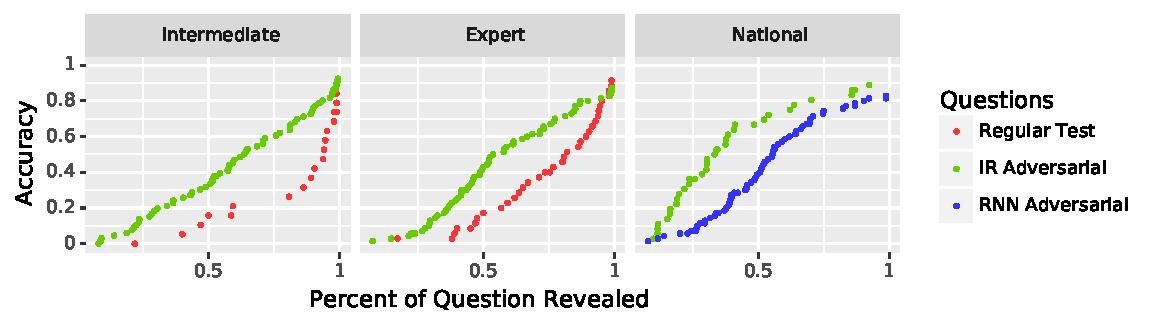
\includegraphics[width=2\columnwidth]{human_breakdown}
\caption{Humans find \challenge{} question about as difficult as
  normal questions: rusty weekend
  warriors (\textit{Intermediate}), active players (\textit{Expert}), or
  the best trivia players in the world (\textit{National}).}
\label{fig:human_breakdown}
\end{figure*}

\begin{figure}[t!]
\centering
\includegraphics[width=0.85\columnwidth]{ikuya_cdf}
\caption{The accuracy of the state-of-the-art Studio Ousia model
  degrades on the \challenge{} questions despite never being directly
  targeted. This verifies that our findings generalize beyond the
  \abr{rnn} and \abr{ir} models.}
\label{fig:ikuya_vs_human}
\end{figure}

In the offline setting (i.e., no pressure to ``buzz'' before an opponent) models
demonstrably struggle on the adversarial questions. But, what happens in
standard \qb{}: live, head-to-head 
games? 

We run two live humans vs. computer matches. The first match uses \abr{ir}
adversarial questions in a forty question, tossup-only \qb{} format. 
We pit a human team of national-level \qb{} players against the
Studio Ousia model~\cite{yamada2018studio},
the current state-of-the-art \qb{} system. The model combines neural,
\abr{ir}, and knowledge graph components (details in Appendix~\ref{sec:ousia}), and won the 2017 \abr{nips} shared task, defeating
a team of expert humans 475--200 on regular \qb{} test questions.
Although the
team at our live event was comparable to the \abr{nips}
2017 team, the tables were turned: the human team won handedly 300--30.

Our second live event is significantly larger: seven human teams play
against models on over 400 questions written adversarially against the
\abr{rnn} model. The human teams range in ability from high school
\qb{} players to national-level teams (Jeopardy! champions, Academic
Competition Federation national champions, top scorers in the World
Quizzing Championships). The models are based on either \abr{ir} or
neural methods. Despite a few close games between the weaker human
teams and the models, humanity prevailed in every
match.\footnote{Videos available at \url{http://trickme.qanta.org}.}

Figures~\ref{fig:human_breakdown}--\ref{fig:ikuya_vs_human} summarize
the live match results for the humans and Ousia model, respectively. Humans
and models have considerably different trends in answer accuracy.
Human accuracy on both regular and adversarial questions rises
quickly in the \emph{last half}
of the question (curves in Figure~\ref{fig:human_breakdown}).
In essence, the ``give-away'' clues at the end of questions are easy for humans to answer.

On the other hand, models on regular test questions
do well in the \emph{first half}, i.e.,
the ``difficult'' clues for humans are easier for models (\emph{Regular Test} in Figure~\ref{fig:ikuya_vs_human}).
However, models, like humans, struggle on 
 adversarial questions in the first half.

\section{Related Work: Knowledge Representation for QA}
\label{sec:bg}

\name{} is impossible without the insights of 
traditional knowledge bases for question answering and question
answering from natural language, which we combine using graph neural
networks.
%
This section describes how we build on these subfields.

\subsection{Knowledge Graph Question Answering}

With knowledge graphs (\abr{kg}) like
Freebase~\cite{bollacker2008freebase} and
DBpedia~\cite{mendes2011dbpedia} enable question answering using their
rich, dependable structure.
%
This has spurred \abr{kg}-specific \abr{qa} datasets on general domain
large scale knowledge graphs: WebQuestions~\cite{berant2013semantic},
SimpleQuestions~\cite{bordes2015large}, and special-domain \abr{kg}s,
such as WikiMovies~\cite{miller2016key}.
%
In turn, these new datasets have prompted special-purpose 
\abr{kgqa} algorithms.
%
Some convert questions to semantic parsing problems and execute the
logical forms on the graph~\cite{cai2013large, kwiatkowski2013scaling,
  reddy2014large, yih2015semantic}.
%
Others use information extraction
 to first extract question related information in \abr{kg}
and then find the answer~\cite{bao2014knowledge, yao2014information,
  gardner2017open}.

These work well on questions tailored for the underlying \abr{kg}.
%
For example,
WebQuestions guarantee its questions can be answered by
Freebase~\cite{berant2013semantic}.
%
Though modern knowledge graphs have good coverage on
entities~\cite{cxthesis}, adding relations takes time and
money~\cite{Paulheim2018HowMI}, often requiring human
effort~\cite{bollacker2008freebase} or scraping human-edited
structured resources~\cite{mendes2011dbpedia}.
%
These lacun\ae represent impede broader use and
adoption.

Like \name{}, \abr{quest}~\cite{Lu:2019:ACQ} seeks to address this by
building a noisy quasi-\abr{kg} with nodes and edges, consisting of
dynamically retrieved entity names and relational phrases from raw
text.
%
Unlike \name{}, this graph is built using existing Open Information
Extraction (\abr{ie}).
%
Then it answers questions on the extracted graph.
%
Unlike \name{}, which is geared toward recall, \abr{ie} errs toward
precision and require regular, clean text.
%
In contrast, many real-world factoid questions contain linguistically
rich structures, making relation extraction challenging.
%
We instead directly extract free-text sentences as indirect relations
between entities, which ensures high coverage of evidence information
to the question.


Similarly, {\abr{graft}-\abr{n}\small et}~\cite{sun2018open} extends an existing \abr{kg} with 
text information.
%
It grafts text evidence onto \abr{kg} nodes but retains the original \abr{kg} relations.
%
It then reasons over this graph to answer \abr{kg}-specific questions.
%
\name{}, in contrast, grafts text evidence onto both nodes and edges
to enrich the relationships between nodes, building on
the success of unconstrained ``machine reading'' \abr{qa} systems.

\subsection{Question Answering over Text}

Compared with highly structured \abr{kg}, unstructured text
collections (e.g., Wikipedia, newswire, or Web scrapes) is cheaper but
noisier for \abr{qa}~\cite{chen2018neural}.
%
Recent datasets such as \squad{}~\cite{rajpurkar2016squad},
\triviaqa{}~\cite{joshi2017triviaqa}, \abr{ms marco}~\cite{marco} and
natural questions~\cite{kwiatkowski2019natural} are typically solved
via a coarse search for a passage (if the passage isn't given) and
then finding a fine-grained span to answer the question.

A rich vein of neural readers match the questions to the given
passages and extract answer spans from them~\cite[inter
  alia]{seo2016bidirectional, yu2018qanet}.  Its popular solutions
include \abr{bidaf}, which matches the question and document passages
by bi-directional attention flows~\cite{seo2016bidirectional},
\abr{qan}{\small et}, which enriches the local contexts with global
self-attention~\cite{yu2018qanet}, and pre-training methods such as
\abr{bert}~\cite{devlin2018bert} and \abr{xln}{\small
  et}~\cite{yang2019xlnet}.

The most realistic models are those that also search for a passage:
%
\drqa{}~\cite{chen2017reading} retrieves documents from Wikipedia and
use \abr{mr} to predict the top span as the answer, and
\abr{orca}~\cite{lee-19} trains the retriever via an inverse cloze
task.
%
Nonetheless, questions mainly answerable by \drqa{} and \abr{orca} only require
single evidence from the candidate sets~\cite{min2018efficient}.
%
\name{} in contrast searches for edge evidence and nodes that can
answer the question; this subgraph often corresponds to the same
documents found by machine reading models.
%
Ideally, it would help synthesize information across \emph{multiple}
passages.


Multi-hop \abr{qa}, where answers require require assembling
information~\citep{welbl2018constructing, yang2018hotpotqa}, is a
\emph{task} to test whether machine reading systems can
synthesize information.
%
\abr{h}{\small otpot}\abr{qa}~\cite{yang2018hotpotqa} is the 
 multi-hop \abr{qa} benchmark: each answer is a text span requiring 
one or two hops.
%
Several models~\cite{qiu-etal-2019-dynamically,
  ding-etal-2019-cognitive, min2019multi} solve
this problem using multiple \abr{mr} models to extract multi-hop
evidence.
%
While we focus on datasets with Wikipedia entities as
answers, expanding \name{} to span-based answers (like \abr{h}{\small otpot}\abr{qa}) is a
natural future direction.



\subsection{Graph Networks for \abr{qa}}

\name{} is not the first to use graph neural networks~\cite[inter
  alia]{scarselli2009graph, kipf2016semi, schlichtkrull2017modeling}
for question answering.
%
\abr{e}{\small ntity}-\abr{gcn}~\cite{de2018question},
\abr{dfgn}~\cite{qiu-etal-2019-dynamically}, and
\abr{hde}~\cite{tu-etal-2019-multi} build the entity graph with entity
co-reference and co-occurrence in documents and apply \abr{gnn} to
the graph to rank the top entity as the answer.
%
\abr{c}{\small og}\abr{qa}~\cite{ding-etal-2019-cognitive} builds the
graph starting with entities from the question, then expanding the
graph using extracted spans from multiple \abr{mr} models as candidate
span nodes and adopt \abr{gnn} over the graph to predict the answer
from span nodes.
%
All these methods' edges are co-reference between entities or binary
scores about their co-occurrence in documents; \name{}'s primary
distinction is using free-text as graph edges which we then represent
and aggregate via a \abr{gnn}.

Other methods have learned representations of relationships between entities.
%
\abr{nubbi}~\cite{chang-09c} used an admixture over relationship
prototypes, while Iyyer et al.~\cite{iyyer-16} used neural dictionary
learning for analyzing literature.
%(including a temporal component for analyzing literature).
%
\name{} draws on these ideas to find similarities between 
passages and questions.



\section{Conclusion}
\label{sec:conc}
We introduce the new problem of noun phrase annotation, which is a generalization of \nel{}. 
We find that introducing noun phrase annotation may be useful in downstream tasks such as question answering. 
However creating a dataset for noun phrase annotation is a difficult task. 
We counter this problem by developing a human-in-the-loop method to efficiently annotate questions and motivate experts to annotate questions by assisting them with studying and directing tournaments. 
To explore the difficulty of noun phrase annotation, we propose experiments that compare the performance of \nel{} and coreference linkers on our noun phrase annotation dataset. 
We additionally design experiments to compare entity linking with multiple configurations in order to determine how best to assist users when entity linking. 
We finally design experiments to determine the effect that noun phrase annotation has upon question answering; we do this by comparing the accuracy of QA models when replacing entities with their entry in the knowledge base. 
Our next steps are to proceed forward with data collection, and to run the experiments on the noun phrase dataset. 

\bibliographystyle{abbrv}
\bibliography{bib/journal-full,bib/pedro}

\end{document}
